\section{FITT-rammeverket}
\label{sec:fitt-rammeverket}

FITT-rammeverket\footnote{Fit between Individuals, Task and Technology} er et system for å lettere kunne analysere og identifisere de sosiotekniske faktorene som påvirker innføringen av nye IT-applikasjoner og -systemer, for dermed å kunne peke på hvilke faktorer det er som hindrer optimal utnyttelse av disse \citep{FITT}.

\noindent
Rammeverket deler settingen IT-systemet skal brukes i, i tre objekter (se figur \ref{FITT-arkitekturen}): (1) $"$Individ$"$, som vil si enkeltbrukere eller brukergrupper av systemet og de som utfører alle oppgaver på arbeidsplassen. (2) $"$Oppgave$"$, helheten av oppgaver og arbeidsprosesser som må utføres av brukeren med den gitte teknologien. (3) $"$Teknologi$"$, som er det tekniske systemet (program- og maskinvare og nettverk) og andre verktøy som individene bruker for å utføre oppgavene.
$"$Organisasjon$"$ blir ikke behandlet som et eget objekt i denne sammenhengen, men kan sees som en del av enten individ-objektet, i den betydning at brukerne jobber i forskjellige roller og grupper i en organisasjon, eller oppgave-objektet, i den betydning at oppgavene og prosessene er organisert på en gitt måte.

\noindent
De tre objektene innehar ulike egenskaper, som kan være tilstede i større eller mindre grad. For et individ kan disse være IT-kunnskap, motivasjon og interesse for oppgaven som skal utføres, fleksibilitet og åpenhet for endringer i arbeidsmåte, team-kultur, organisatorisk kontekst, sammarbeidet innenfor team og politikk i en organisasjon. For en oppgave kan det være organisering av oppgavene som skal gjennomføres, gjensidig avhengighet mellom oppgavene og oppgavenes grad av kompleksitet. Teknologi kan ha egnskaper som stabilitet og brukbarhet, verktøyets kostnad, funksjonalitet, tilgjengelig teknisk infrastruktur, integrasjon av verktøy og verktøy tilgjengelig i en gitt klinisk situasjon.

\begin{figure}[H]
\centering
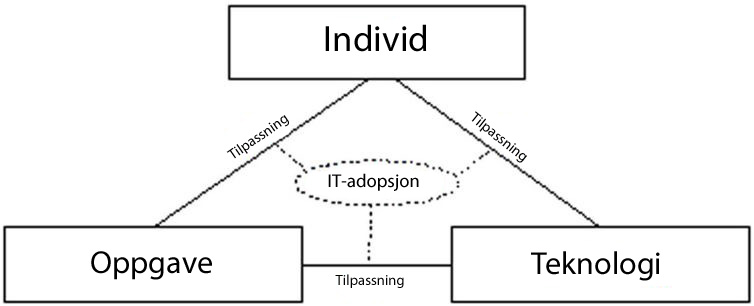
\includegraphics[scale=0.4]{FITT_norsk.jpg}
\caption{FITT-arkitekturen \citep{FITT} (oversatt av forfatterne)}
\label{FITT-arkitekturen}
\end{figure}

\noindent
Fokuset for rammeverket er samspillet mellom objektene (og deres egenskaper), hvordan de passer (fit) sammen, og ikke objektene i seg selv. Med denne tilnærmingen kan målet med IT-ledelse defineres som det å finne en optimal tilpasning (fit) mellom bruker, oppgave og teknologi. Dersom objektene mangler, eller har lite utviklede egenskaper som er nødvendig for et optimalt samspill, kan man direkte påvirke egenskapene til det enkelte objektet. Et eksempel er manglende IT-kunnskap blant brukerne (individ), hvor opplæring av ansatte kan øke tilstedeværelsen av denne egenskapen. Siden dette er tiltak som påvirker objektene direkte, har det også en indirekte påvirkning på samspillet mellom dem.

\noindent
Det vil alltid finnes eksterne faktorer som er vanskelig eller umulig å påvirke, som høy turnover, eller nye lover og regler. Disse faktorene fører til at det aldri vil oppstå en statisk situasjon med hensyn på de tre dimensjonene av samspill, og derfor heller ikke optimaliseringen av disse.

\noindent
Ved å bruke dette rammeverket kan man lettere se hvor eventuelle problemer ved innføringen av systemet ligger. En vanlig feiltolkning er at problemer som ligger i samspillet mellom bruker og oppgave blir tillagt teknologien. Et eksempel på dette er dersom innføringen av et nytt IT-system gir brukerne flere dokumentasjonssoppgaver. Ofte vil det nye systemet få skylden for dette, mens problemet ligger i brukernes misnøye med oppgaven, og ikke nødvendigvis teknologien i seg selv.

